\باب{تفرق}
گزشتہ باب میں ہم نے دیکھا کہ کسی نقطہ پر سیکنٹ کی ڈھلوان کی حد کو اس نقطے پر منحنی کی ڈھلوان کہتے ہیں۔ یہ حد، جس کو تفرق کہتے ہیں، تفاعل تبدیل ہونے کی شرح کی ناپ ہے جو احصاء میں اہم ترین تصورات میں سے ایک ہے۔تفرق کو سائنس، معاشیات اور دیگر شعبوں میں بہت زیادہ استعمال کیا جاتا ہے جہاں سمتی رفتار اور اسراع کا حساب، مشین کی کارکردگی سمجھنے، وغیرہ کے لئے اس کو استعمال میں لایا جاتا ہے۔تفرق کو حد سے تلاش کرنا مشکل کام ہے۔اس باب میں تفرق حاصل کرنے کے طریقوں پر غور کیا جائے گا۔ 

\حصہ{تفاعل کا تفرق}
گزشتہ باب کے آخر میں ہم نے نقطہ \عددی{x=x_0} پر منحنی \عددی{y=f(x)} کی ڈھلوان \عددی{m} کی درج ذیل تعریف پیش کی۔
\begin{align*}
m=\lim_{h\to 0}\frac{f(x_0+h)-f(x_0)}{h}
\end{align*} 
اس حد کو، بشرطیکہ یہ موجود ہو، \عددی{x_0} پر \عددی{f} کا تفرق کہتے ہیں۔اس حصے میں \عددی{f} کی دائرہ کار میں ہر نقطے پر \عددی{f} کی ڈھلوان پر  بطور تفاعل غور کیا جائے گا۔

\ابتدا{تعریف}
متغیر \عددی{x} کے لحاظ سے تفاعل \عددی{f} کا \اصطلاح{تفرق}\فرہنگ{تفرق}\حاشیہب{derivative}\فرہنگ{derivative} درج ذیل  تفاعل \عددی{f'} ہے، بشرطیکہ یہ حد موجود ہو۔
\begin{align*}
f'(x)=\lim_{h\to 0}\frac{f(x+h)-f(x)}{h}
\end{align*}
\انتہا{تعریف}
%===========================

\عددی{f'} کا دائرہ کار، نقطوں کا وہ سلسلہ جہاں یہ حد موجود ہو، تفاعل \عددی{f} کے دائرہ کار سے کم ہو سکتا ہے۔ اگر \عددی{f'(x)} موجود ہو تب ہم کہتے ہیں کہ \عددی{x} پر \عددی{f} کا \اصطلاح{تفرق} پایا جاتا ہے یا کہ \عددی{x} پر \عددی{f} \اصطلاح{قابل تفرق}\فرہنگ{تفرق!قابل}\حاشیہب{differentiable}\فرہنگ{differentiable} ہے۔

\جزوحصہء{علامتیت}
تفاعل \عددی{y=f(x)} کی تفرق کو ظاہر کرنے کے کئی طریقے رائج ہیں۔\عددی{f'(x)} کے علاوہ درج ذیل علامتیں کافی مقبول ہیں۔
\begin{description}
\جزو{$y'$}
یہ مختصر علامت ہے جو غیر تابع متغیر کی نشاندہی نہیں کرتی ہے۔
\جزو{$\tfrac{\dif y}{\dif x}$}
یہ علامت دونوں متغیرات کی نشاندہی کرتی ہے اور تفرق کو \عددی{\dif} سے ظاہر کرتی ہے۔  
\جزو{$\tfrac{\dif f}{\dif x}$}
یہ علامت تفاعل کا نام واضح کرتی ہے۔
\جزو{$\tfrac{\dif}{\dif x} f(x)$}
اس علامت سے ظاہر ہوتا ہے کہ تفرق کا عمل \عددی{f} پر لاگو کیا جاتا ہے (شکل \حوالہ{شکل_تفرق_ڈبہ_صورت})۔
\جزو{$D_xf$}
یہ تفرقی عامل ہے۔
\جزو{$\dot{y}$} 
نیوٹن اس علامت کو استعمال کرتے تھے جو اب وقتی تفرق کو ظاہر کرنے کے لئے استعمال کیا جاتا ہے۔
\end{description} 

ہم \عددی{\tfrac{\dif y}{\dif x}} کو "\عددی{x} کے لحاظ سے \عددی{y} کو تفرق" پڑھتے ہیں۔اسی طرح \عددی{\tfrac{\dif f}{\dif x}} اور \عددی{\tfrac{\dif}{\dif x}f(x)} کو "\عددی{x} کے لحاظ سے \عددی{f} کا تفرق" پڑھا جاتا ہے۔
\begin{figure}
\centering
\begin{tikzpicture}
\draw(0,0) rectangle ++(2,1);
\draw[latex-](0,0.5)--++(-2,0)node[pos=0.5,above,align=center]{\RL{داخلی تفاعل}\\  $y=f(x)$};
\draw[-latex](2,0.5)--++(2,0)node[pos=0.5,above,align=center]{\RL{خارجی تفرق}\\ $y'=\tfrac{\dif f}{\dif x}$};
\draw(1,0.5)node[align=center]{\RL{عمل تفرق}\\ $\tfrac{\dif}{\dif x}$};
\end{tikzpicture}
\caption{تفرق کے عمل کی ڈبہ صورت}
\label{شکل_تفرق_ڈبہ_صورت}
\end{figure}

\جزوحصہء{تفرق کی تعریف سے تفرق کا حصول}
مثال \حوالہ{مثال_حد_سیدھا_خط_الف} اور مثال \حوالہ{مثال_حد_ڈھلوان} میں تفاعل \عددی{y=mx+b} اور \عددی{y=\tfrac{1}{x}} کے تفرق کو تعریف سے حاصل کرنا دکھایا گیا۔مثال \حوالہ{مثال_حد_سیدھا_خط_الف} میں 
\begin{align*}
\frac{\dif}{\dif x}(mx+b)=m
\end{align*}
اور   مثال \حوالہ{مثال_حد_ڈھلوان} میں
\begin{align}
\frac{\dif}{\dif x}\big(\frac{1}{x}\big)=-\frac{1}{x^2}
\end{align}
حاصل کیا گیا۔

\موٹا{تفرق کی تعریف سے  تفرق کے حاصل کے اقدام} 
\begin{enumerate}[1.]
\item
\عددی{f(x)} اور \عددی{f(x+h)} لکھیں۔
\item
درج ذیل تفریقی حاصل تقسیم کو پھیلا کر اس کی سادہ ترین صورت حاصل کریں۔
\begin{align*}
\frac{f(x+h)-f(x)}{h}
\end{align*}
\item
سادہ ترین حاصل تقسیم سے \عددی{f'(x)} حاصل کرنے کی خاطر درج ذیل حد تلاش کریں۔
\begin{align*}
f'(x)=\lim_{h\to 0}\frac{f(x+h)-f(x)}{h}
\end{align*}
\end{enumerate}

مزید دو مثال درج ذیل ہیں۔

\ابتدا{مثال}\شناخت{مثال_تفرق_حصول_بذریعہ_تعریف_الف}
\begin{enumerate}[a.]
\item
\عددی{f(x)=\tfrac{x}{x-1}} کو تفرق کریں۔
\item
تفاعل \عددی{y=f(x)} کی ڈھلوان کس نقطے پر \عددی{-1} کے برابر ہے؟
\end{enumerate}
حل:\quad  (ا) \quad  ہم مذکورہ بالا تین اقدام استعمال کرتے ہوئے تعریف سے تفرق حاصل کرتے ہیں۔\\
\موٹا{پہلا قدم:} یہاں \عددی{f(x)=\tfrac{x}{x-1}} ہے جس سے \عددی{f(x+h)=\tfrac{x+h}{(x+h)-1}} لکھا جا سکتا ہے۔\\
\موٹا{دوسرا قدم:}
\begin{align*}
\frac{f(x+h)-f(x)}{h}&=\frac{\tfrac{x+h}{x+h-1}-\tfrac{x}{x-1}}{h}\\
&=\frac{1}{h}\cdot \frac{(x+h)(x-1)-x(x+h-1)}{(x+h-1)(x-1)}\\
&=\frac{1}{h}\cdot \frac{-h}{(x+h-1)(x-1)}
\end{align*}
\موٹا{تیسرا قدم:}
\begin{align*}
f'(x)&=\lim_{h\to 0} \frac{-1}{(x+h-1)(x-)}=-\frac{1}{(x-1)^2}
\end{align*}
(ب) \quad \عددی{y=f(x)} کی ڈھلوان اس صورت \عددی{-1} کے برابر ہو گی جب درج ذیل ہو۔
\begin{align*}
-\frac{1}{(x-1)^2}=-1
\end{align*}
اس مساوات \عددی{(x-1)^2=1} کے مترادف ہے لہٰذا  \عددی{x=2} اور \عددی{x=0} درکار نتائج ہیں (شکل  \حوالہ{شکل_مثال_تفرق_حصول_بذریعہ_تعریف_الف})۔
\begin{figure}
\centering
\begin{tikzpicture}
\begin{axis}[small,axis lines=middle,xlabel={$x$},ylabel={$y$},xtick={1,2},ytick={2},xlabel style={at={(current axis.right of origin)},anchor=west}]
\addplot[domain=-3:0.75,samples=50]{x/(x-1)};
\addplot[domain=1.25:4]{x/(x-1)}node[pos=0.15,right]{$y=\tfrac{x}{x-1}$};
\draw[shorten <=-1.5cm, shorten >=-0.5cm](axis cs:0,0)node[circ]{}node[below left]{$(0,0)$}--(axis cs:1,-1);
\draw[shorten <=-1.5cm](axis cs:2,2)node[circ]{}node[below left]{$(2,2)$}--(axis cs:3,1);
\draw[dashed] (axis cs:1,-3)--(axis cs:1,5);
\draw(axis cs:-1.75,1.5)node[above]{$m=-1$};
\draw(axis cs:3,1)node[below]{$m=-1$};
\end{axis}
\end{tikzpicture}
\caption{
\عددی{x=0} اور \عددی{x=2} پر \عددی{y'=-1} ہو گا (مثال \حوالہ{مثال_تفرق_حصول_بذریعہ_تعریف_الف})۔
}
\label{شکل_مثال_تفرق_حصول_بذریعہ_تعریف_الف}
\end{figure}
\انتہا{مثال}
%=====================
\ابتدا{مثال}\شناخت{مثال_تفرق_حصول_بذریعہ_تعریف_ب}
\begin{enumerate}[1.]
\item
\عددی{x>0} کے لئے \عددی{y=\sqrt{x}} کا تفرق حاصل کریں۔
\item
\عددی{x=4} پر تفاعل \عددی{y=\sqrt{x}} کے مماس کی مساوات حاصل کریں۔
\end{enumerate}
حل:\quad
(ا) \quad \موٹا{پہلا قدم:}\quad
\begin{align*}
f(x)=\sqrt{x},\quad f(x+h)=\sqrt{x+h}
\end{align*}
\موٹا{دوسرا قدم:}
\begin{align*}
\frac{f(x+h)-f(h)}{h}&=\frac{\sqrt{x+h}-\sqrt{x}}{h}&& \text{\RL{$\tfrac{\sqrt{x+h}+\sqrt{x}}{\sqrt{x+h}+\sqrt{x}}$ سے ضرب دیتے ہیں}}\\
&=\frac{(x+h)-x}{h(\sqrt{x+h}+\sqrt{x})}\\
&=\frac{1}{\sqrt{x+h}+\sqrt{x}}
\end{align*}
\موٹا{تیسرا قدم:}
\begin{align*}
f'(x)&=\lim_{h\to 0}\frac{1}{\sqrt{x+h}+\sqrt{x}}=\frac{1}{2\sqrt{x}}
\end{align*}
شکل \حوالہ{شکل_مثال_تفرق_حصول_بذریعہ_تعریف_ب} دیکھیں۔\\
(ب)\quad
\عددی{x=4} پر تفاعل کی ڈھلوان درج ذیل ہے۔
\begin{align*}
\frac{\dif y}{\dif x}|_{x=4}=\frac{1}{2\sqrt{x}}|_{x=4}=\frac{1}{4}
\end{align*}
نقطہ \عددی{(4,2)} سے گزرتا ہوا خط جس کی ڈھلوان \عددی{\tfrac{1}{4}} ہو \عددی{(4,2)} پر \عددی{f} کا مماس ہو گا۔مماس کی مساوات حاصل کرتے ہیں۔
\begin{align*}
y&=2+\frac{1}{4}(x-4)=\frac{1}{4}x+1
\end{align*}
%
\begin{figure}
\centering
\begin{subfigure}{0.5\textwidth}
\centering
\begin{tikzpicture}
\begin{axis}[clip=false,small,axis lines=middle,xlabel={$x$},ylabel={$y$},ymin=-0.3,xtick={\empty},ytick={\empty}]
\addplot[domain=0:0.5]{sqrt(x)};
\addplot[domain=0.5:8]{sqrt(x)}node[pos=0.8,sloped, below]{$y=\sqrt{x}$};
\draw[shorten <=-2.5cm,shorten >=-1.5cm](axis cs:4,2)node[circ]{}--(axis cs:5,2.25)node[pos=1,sloped,above]{$m=\tfrac{1}{2\sqrt{x}}$};
\draw[dashed](axis cs:4,2)--(axis cs:4,0)node[circ]{}node[below]{$x$};
\end{axis}
\end{tikzpicture}
\caption{تفاعل \عددی{y=\sqrt{x}}}
\end{subfigure}%
\begin{subfigure}{0.5\textwidth}
\centering
\begin{tikzpicture}
\begin{axis}[small,axis lines=middle,xlabel={$x$},ylabel={$y'$},xtick={\empty},ytick={\empty},xmin=0,ymin=-0.3,ylabel style={at={(current axis.above origin)},anchor=south}]
\addplot[domain=0.25:8,samples=50]{1/(2*sqrt(x))}node[pos=0.8,sloped, above]{$y'=\tfrac{1}{2\sqrt{x}}$};
\draw[dashed](axis cs:4,0.25)node[circ]{}--(axis cs:4,0)node[circ]{}node[below]{$x$};
\end{axis}
\end{tikzpicture}
\caption{
\عددی{x>0} کے لئے  \عددی{y'=\tfrac{1}{2\sqrt{x}}}
}
\end{subfigure}
\begin{subfigure}{0.55\textwidth}
\centering
\begin{tikzpicture}
\begin{axis}[clip=false,small,axis lines=middle,xlabel={$x$},ylabel={$y$},ymin=-0.3,xtick={4},ytick={1,2},xmin=-1]
\addplot[domain=0:0.5]{sqrt(x)};
\addplot[domain=0.5:8]{sqrt(x)}node[pos=0.8,sloped, below]{$y=\sqrt{x}$};
\draw[shorten <=-3cm,shorten >=-1.75cm](axis cs:4,2)node[circ]{}node[below,xshift={1mm}]{$(4,2)$}--(axis cs:5,2.25)node[pos=1,sloped,above right]{$y=\tfrac{1}{4}x+1$};
\end{axis}
\end{tikzpicture}
\caption{
تفاعل \عددی{y=\sqrt{x}} اور نقطہ \عددی{(4,2)} پر اس کا مماس \عددی{y=\tfrac{1}{4}x+1}۔
}
\end{subfigure}
\caption{اشکال برائے مثال \حوالہ{مثال_تفرق_حصول_بذریعہ_تعریف_ب}۔نقطہ \عددی{x=0} پر تفاعل معین ہے لیکن اس کا تفرق غیر معین ہے۔}
\label{شکل_مثال_تفرق_حصول_بذریعہ_تعریف_ب}
\end{figure}
\انتہا{مثال}

نقطہ \عددی{x=a} پر تفاعل \عددی{y=f(x)} کے تفرق کی قیمت حاصل کرنے کو
\begin{align*}
f'(a)=\lim_{h\to 0}\frac{f(a+h)-f(a)}{h}
\end{align*}
کے علاوہ
\begin{align*}
\left. y' \right \vert_{x=a}=\left. \frac{\dif y}{\dif x} \right\vert_{x=a}=\left. \frac{\dif}{\dif x}f(x) \right\vert_{x=a}
\end{align*}
سے بھی ظاہر کیا جا سکتا ہے جہاں \عددی{|_{x=a}} علامت کی بائیں ہاتھ کی قیمت کو \عددی{x=a} پر حاصل کیا جاتا ہے۔ 
%======================

\جزوحصہء{اندازاً حاصل قیمتوں سے \عددی{f'} کی ترسیم}
تفاعل \عددی{y=f(x)} کی تجربہ سے حاصل قیمتوں (مثلاً دباو بالمقابل وقت یا آبادی بالمقابل وقت) کو ہم بطور نقطے ترسیم کرنے کے بعد عموماً سیدھے خطوط یا ہموار منحنی سے جوڑتے ہیں تا کہ ہمیں \عددی{f} کی صورت نظر آئے۔مختلف مقامات پر تفاعل کی ڈھلوان \عددی{f'} سے ہم عموماً \عددی{f'} کو بھی ترسیم کر پاتے ہیں۔درج ذیل مثال میں اس عمل کو دکھایا گیا ہے۔

\ابتدا{مثال}\شناخت{مثال_تفرق_پرواز}\موٹا{دوا}\\
\عددی{23} اپریل \سن{1988} کو \عددی{31} کلوگرام وزنی،  \ترچھا{ڈیڈلس}\حاشیہد{Daedalus} نامی جہاز کو انسانی جسمانی طاقت سے   یونان کے جنوب مشرق میں جزیرہ \ترچھا{کریتی}\حاشیہد{Crete} سے جزیرہ \ترچھا{سانٹورینی}\حاشیہد{Santorini} تک اڑا کر \عددی{115.11} کلومیٹر  کا فاصلہ \عددی{3} گھنٹوں اور \عددی{54} منٹوں میں طے کرتے ہوئے عالمی کارنامہ سرانجام دیا گیا۔یہ جہاز امریکی یونیورسٹی\حاشیہد{MIT} کے طلبہ نے تیار کیا۔ اس تاریخی پرواز کی تیاری کے لئے ممکنہ ہوا بازوں کی جسمانی برداشت کو \عددی{6} گھنٹوں تک پرکھا جاتا تھا جس دوران ماہرین ہوا بازوں  کی کثافت دموی شکر پر نظر رکھتے تھے۔ان میں سے ایک ہوا باز کی کثافت دموی شکر (ملی گرام فی ڈیسی لٹر) بالمقابل وقت (گھنٹوں) کو شکل \حوالہ{شکل_مثال_تفرق_پرواز}-ا میں دکھایا گیا ہے۔
\begin{figure}
\centering
\begin{subfigure}{0.5\textwidth}
\centering
\begin{tikzpicture}[x=0.5cm,y=0.5cm]
\foreach \y/\ys in {1/80,2/90,3/100,4/110}{\draw[gray](0,\y)node[left,black]{$\ys$}--++(7,0);}
\foreach \x in {1,2,3,4,5,6}{\draw[gray](\x,0)node[below,black]{$\x$}--++(0,5);}
\draw[-latex](-0.25,0)--(7,0)node[right]{$t\,(\si{\hour})$};
\draw[-latex](0,-0.2)--(0,5)node[above]{$y\,(\si{\milli\gram\per\deci\litre})$};
\draw(0,0.9)--(1,2.25)--(2,3.85)--(3,3.25)--(4,2.3)--(5,2.5)--(6,2.5);
\end{tikzpicture}
\caption{}
\end{subfigure}%
\begin{subfigure}{0.5\textwidth}
\centering
\begin{tikzpicture}[x=0.5cm,y=0.5cm]
\draw[-latex](-0.25,0)--(7,0)node[right]{$t\,(\si{\hour})$};
\draw[-latex](0,-2.5)--(0,4)node[above]{$y'\,(\tfrac{\si{\milli\gram\per\deci\litre}}{\si{\hour}})$};
\foreach \y/\ys in {-2/-10,-1/-5,1/5,2/10,3/15}{\draw(0,\y)node[left]{$\ys$}--++(0.2,0);}
\foreach \x in {1,2,3,4,5,6}{\draw(\x,0)node[below]{$\x$}--++(0,0.2);}
\draw[thick](0,2.786)--++(1,0);
\draw[thick](1,3)--++(1,0);
\draw[thick](2,-1.572)--++(1,0);
\draw[thick](3,-1.71)--++(1,0);
\draw[thick](4,0.428)--++(1,0);
\draw[thick](5,0.02)--++(1,0);
\end{tikzpicture}
\caption{}
\end{subfigure}%
\caption{(ا) قبل پرواز پرکھ برداشت کے دوران دموی شکر (ب) دموی شکر کا ڈھلوان مختلف پرکھ میں نہایت تیزی سے بہت زیادہ تبدیل ہوتا ہے۔}
\label{شکل_مثال_تفرق_پرواز}
\end{figure}
موادی نقطوں کو قطعات سے جوڑ کر ترسیم حاصل کی گئی ہے۔ہر قطع کی غیر متغیر ڈھلوان سے اس قطع پر کثافت دموی شکر کے تفرق کا اندازہ کیا جا سکتا ہے۔ تمام قطعات پر اس تفرق کو حاصل کرتے ہوئے شکل \حوالہ{شکل_مثال_تفرق_پرواز}-ب میں ترسیم کیا گیا ہے۔مثال کے طور پر پہلے گھنٹہ میں کثافت دموی شکر \عددی{\SI{79}{\milli\gram\per\deci\litre}} سے بڑھ کر \عددی{\SI{83}{\milli\gram\per\deci\litre}} ہو جاتا ہے۔یوں  تبدیل \عددی{\Delta y=93-79=\SI{14}{\milli\gram\per\deci\litre}} ہے جس کو \عددی{\Delta x=\SI{1}{\hour}} سے تقسیم کرتے ہوئے پہلے گھنٹہ میں کثافت کی شرح تبدیلی  
\begin{align*}
\frac{\Delta y}{\Delta x}=\frac{14}{1}=\frac{\SI{14}{\milli\gram\per\deci\litre}}{\si{\hour}}
\end{align*}    
حاصل ہوتی ہے۔

دھیان رہے کہ لمحات \عددی{t=1,2,\cdots,5} پر، جہاں ترسیم کے کونے پائے جاتے ہیں لہٰذا ہم ڈھلوان حاصل نہیں کر سکتے ہیں، ہم کثافت کی شرح تبدیلی کا اندازہ نہیں لگا سکتے ہیں۔ان نقطوں پر تفرقی سیڑھی تفاعل غیر معین ہے۔   
\انتہا{مثال}
%=========================

جہاں ہمارے پاس اتنے زیادہ تعداد میں نقطے ہوں کہ انہیں قطعات سے جوڑ کر ہموار منحنی حاصل ہوتی ہو وہاں ہم تفرق کو بھی ہموار خط سے ظاہر کرنا چاہیں گے۔اگلے مثال میں ایسا ہی کیا گیا ہے۔

\ابتدا{مثال}\شناخت{مثال_تفرق_ہموار_منحنی_الف}
تفاعل \عددی{y=f(x)} کو شکل \حوالہ{شکل_مثال_تفرق_ہموار_منحنی_الف}-ا میں دکھایا گیا ہے۔اس کے تفرق \عددی{y'=f'(x)} کو ترسیم کریں۔
\begin{figure}
\centering
\begin{subfigure}{0.5\textwidth}
\centering
\begin{tikzpicture}[declare function={
f(\x)=(\x+2)*(\x-1)*(\x-5);
dfdx(\x)=3*\x*\x-8*\x-7;
}]
\begin{axis}[clip=false,grid=both,grid style={draw=gray},small,axis lines=middle,xlabel={$x$},ylabel={$y=f(x)$},xmin=-1.5,ymin=-22,ymax=29,xtick={-1,1,2,3,4,5},,xticklabels={,$1$,$2$,$3$,$4$,},xlabel style={at={(current axis.right of origin)},anchor=west}]
\addplot[domain=-1:5.57]{f(x)};
\draw[shorten <=-0.5cm](axis cs:-0.69425,12.597)node[circ]{}node[above]{$A$};
\draw[](axis cs:0.4514,6.117)node[circ]{}node[above]{$B$};
\draw[](axis cs:1.333,-4.07)node[circ]{}node[above]{$C$};
\draw[](axis cs:3.36092,-20.745)node[circ]{}node[above]{$D$};
\draw[](axis cs:4.616,-9.186)node[circ]{}node[left]{$E$};
%
\addplot[domain=-0.69425-0.5:-0.69425+0.5]{12.597+dfdx(-0.69425)*(x-(-0.69425))};
\addplot[domain=0.4514-0.5:0.4514+0.5]{6.117+dfdx(0.4514)*(x-0.4514)};
\addplot[domain=3.36092-0.7:3.36092+0.7]{-20.745+dfdx(3.36092)*(x-3.36092)};
\addplot[domain=4.0753:5.0753]{-9.186+dfdx(4.616)*(x-4.616)};
%
\draw[thick](axis cs:4.0753,-20)--(axis cs:5.0753,-20)node[pos=0.5,pin=-45:{$\Delta x=1$}]{}--(axis cs:5.0753,0)node[pos=0.35,right,fill=white]{$\Delta y=20$};
\end{axis}
\end{tikzpicture}
\caption{دیا گیا تفاعل \عددی{y=f(x)}}
\end{subfigure}%
\begin{subfigure}{0.5\textwidth}
\centering
\begin{tikzpicture}[declare function={
f(\x)=(\x+2)*(\x-1)*(\x-5);
dfdx(\x)=3*\x*\x-8*\x-7;
}]
\begin{axis}[grid=both,grid style={draw=gray},small,axis lines=middle,xlabel={$x$},ylabel={$y'=f'(x)$},ymin=-15,ymax=29,xmin=-1.5,xmax=5.5,xtick={-1,1,2,3,4,5},xticklabels={,$1$,$2$,$3$,$4$,}]
\addplot[domain=-1:5.57]{dfdx(x)};
\draw[](axis cs:-0.694,0)node[circ]{}node[above,xshift={2mm}]{$A'$};
\draw[](axis cs:0.4514,-10)node[circ]{}node[above]{$B'$};
\draw[](axis cs:1.333,-12)node[circ]{}node[above]{$C'$};
\draw[](axis cs:3.36092,0)node[circ]{}node[above]{$D'$};
\draw[](axis cs:4.616,20)node[circ]{}node[left]{$E'$};
\end{axis}
\end{tikzpicture}
\caption{دیے گئے تفاعل کا تفرق \عددی{y'=f'(x)}}
\label{}
\end{subfigure}%
\caption{اشکال برائے مثال \حوالہ{شکل_مثال_تفرق_ہموار_منحنی_الف}}
\label{شکل_مثال_تفرق_ہموار_منحنی_الف}
\end{figure}

حل:\quad
شکل \حوالہ{شکل_مثال_تفرق_ہموار_منحنی_الف}-ا کے ترسیم پر مختلف نقطوں مثلاً \عددی{A,B,C,D,E} پر منحنی کی ڈھلوان جیومیٹریائی طریقے سے حاصل کرتے ہیں۔شکل-ا کو دیکھ کر ہی وہ خطے نظر آتے ہیں جہاں ڈھلوان مثبت، منفی اور صفر ہیں۔ \عددی{A} سے \عددی{D} تک ڈھلوان منفی ہے جبکہ  \عددی{D} کی دائیں جانب اور \عددی{A} کی بائیں جانب  ڈھلوان مثبت ہے۔اسی طرح وہ خطے بھی واضح ہیں جہاں ڈھلوان بڑھ یا گھٹ رہا ہے۔نقطہ \عددی{A} اور \عددی{D} پر سیکنٹ کی حد کی ڈھلوان \عددی{0} ہیں جو شکل \حوالہ{شکل_مثال_تفرق_ہموار_منحنی_الف}-ب کے مطابقتی نقطے \عددی{A'} اور \عددی{D'} دیتے ہیں جہاں \عددی{y'=0} ہے۔نقطہ \عددی{E} پر سیکنٹ کی ڈھلوان حاصل کرنے کی خاطر قائمہ مثلث مکمل کیا گیا ہے جہاں سے \عددی{\Delta x=1} اور \عددی{\Delta y=20} پڑھے جا سکتے ہیں جن سے \عددی{\tfrac{\Delta y}{\Delta x}=20} حاصل ہوتا ہے۔شکل-ب میں اس کو نقطہ \عددی{E'} دکھایا گیا ہے۔آپ شکل-ا میں نقطہ \عددی{B} پر بھی مثلث بنا کر ڈھلوان حاصل کر سکتے ہیں جو \عددی{-10} ہو گا جس کو شکل-ب میں \عددی{B'} دکھایا گیا ہے۔شکل-ا میں نقطہ \عددی{C} وہ نقطہ ہے جس پر ڈھلوان کی کم تر قیمت حاصل ہوتی ہے جس سے شکل-ب کا نشیب \عددی{C'} حاصل ہوتا ہے۔  
\انتہا{مثال}
%======================

\جزوحصہء{وقفے پر قابل تفرق؛ یک طرفہ تفرق}
کھلے وقفہ (متناہی یا لا متناہی) پر تفاعل \عددی{y=f(x)} اس صورت قابل تفرق ہو گا جب اس وقفے کے ہر نقطے پر \عددی{f} قابل تفرق ہو۔یہ بند وقفہ \عددی{[a,b]} پر اس صورت قابل تفرق ہو گا جب اس وقفے کے ہر اندرونی نقطے پر \عددی{f} قابل تفرق ہو اور درج ذیل تفرق موجود ہوں (شکل \حوالہ{شکل_تفرق_آخری_سر_تفرق_یک_طرفہ})۔
\begin{align*}
\lim_{h\to 0^+}\frac{f(a+h)-f(a)}{h}&&\text{\RL{\عددی{a} پر دائیں ہاتھ تفرق}}\\
\lim_{h\to 0^-}\frac{f(b+h)-f(b)}{h}&&\text{\RL{\عددی{b} پر بائیں ہاتھ تفرق}}
\end{align*}
%
\begin{figure}
\centering
\begin{minipage}{0.45\textwidth}
\centering
\begin{tikzpicture}[declare function={f(\x)=1.5-sin(deg(\x)); dfdx(\x)=-cos(deg(\x));}]
\pgfmathsetmacro{\xA}{pi/4}
\pgfmathsetmacro{\xB}{pi/2+pi/6}
\pgfmathsetmacro{\xC}{3/2*pi-pi/8}
\pgfmathsetmacro{\xD}{2*pi-pi/3}
\pgfmathsetmacro{\yA}{f(\xA)}
\pgfmathsetmacro{\yB}{f(\xB)}
\pgfmathsetmacro{\yC}{f(\xC)}
\pgfmathsetmacro{\yD}{f(\xD)}
\pgfmathsetmacro{\mA}{dfdx(\xA)}
\pgfmathsetmacro{\mD}{dfdx(\xD)}
\begin{axis}[axis y line=none,clip=false,small,axis lines=middle,xlabel={$x$},ylabel={$y$},xmin=0,ymin=0,xtick={\xA,\xB,\xC,\xD},xticklabels={$a$,$a+h$,$b+h$,$b$},xmax=6.3,ytick={\empty}]
\addplot[domain=\xA:\xD,samples=100]{f(x)}node[pos=0.4,right,font=\scriptsize]{$y=f(x)$};
\draw[shorten <=-0.5cm, shorten >=-0.5cm](axis cs:\xA,\yA)--(axis cs:\xB,\yB);
\draw[shorten <=-0.5cm, shorten >=-0.5cm](axis cs:\xC,\yC)--(axis cs:\xD,\yD);
\draw[dashed](axis cs:\xA,0)--(axis cs:\xA,\yA);
\draw[dashed](axis cs:\xB,0)--(axis cs:\xB,\yB);
\draw[dashed](axis cs:\xC,0)--(axis cs:\xC,\yC);
\draw[dashed](axis cs:\xD,0)--(axis cs:\xD,\yD);
\addplot[thick,domain=\xA-pi/6:\xA+pi/4]{\yA+\mA*(x-\xA)}node[pos=0,above,yshift=-2mm,align=left]{\RL{$=$ ڈھلوان}\\ $\lim\limits_{h\to 0^+}\tfrac{f(a+h)-f(a)}{h}$};
\addplot[thick,domain=\xD-pi/4:\xD+pi/4]{\yD+\mD*(x-\xD)}node[pos=0,above,yshift=-2mm,align=left]{\RL{$=$ ڈھلوان}\\ $\lim\limits_{h\to 0^-}\tfrac{f(b+h)-f(b)}{h}$};
\draw(axis cs:\xB,0)node[below,yshift=-4mm,font=\scriptsize]{$h>0$};
\draw(axis cs:\xC,0)node[below,yshift=-4mm,font=\scriptsize]{$h<0$};
\end{axis}
\end{tikzpicture}
\caption{وقفہ کے آخری سر نقطوں پر تفرق یک طرفہ ہوں گے۔}
\label{شکل_تفرق_آخری_سر_تفرق_یک_طرفہ}
\end{minipage}\hfill
\begin{minipage}{0.45\textwidth}
\centering
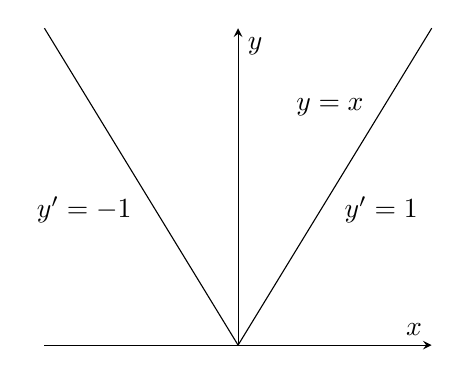
\begin{tikzpicture}
\begin{axis}[clip=false,small,axis lines=middle,xlabel={$x$},ylabel={$y$},xtick={\empty},ytick={\empty}]
\addplot[domain=-4:0]{-x}node[pos=0.5,below left]{$y'=-1$};
\addplot[domain=0:4]{x}node[pos=0.5,below right]{$y'=1$};
\draw(axis cs:1,3)node[right]{$y=\abs{x}$};
\end{axis}
\end{tikzpicture}
\caption{چونکہ مبدا پر بائیں ہاتھ اور دائیں ہاتھ تفرق مختلف ہیں لہٰذا مبدا پر تفاعل کا تفرق غیر موجود ہے (مثال \حوالہ{مثال_تفرق_مبدا_پر_غیر_موجود})۔}
\label{شکل_مثال_تفرق_مبدا_پر_غیر_موجود}
\end{minipage}
\end{figure}

تفاعل کے دائرہ کار میں کہیں پر بھی تفاعل کے دائیں ہاتھ اور بائیں ہاتھ تفرق  معین ہو سکتے ہیں۔یک طرفہ اور دو طرفہ حد کا تعلق ان تفرق پر بھی قابل اطلاق ہو گا۔  مسئلہ \حوالہ{مسئلہ_حد_یک_طرفہ_بالمقابل_دو_طرفہ_حد} کی بنا کسی نقطے پر تفاعل کا تفرق صرف اور صرف اس صورت موجود ہو گا جب اس نقطے پر تفاعل کے بائیں ہاتھ تفرق اور دائیں ہاتھ تفرق موجود ہوں اور ایک دوسرے کے برابر ہوں۔

\ابتدا{مثال}\شناخت{مثال_تفرق_مبدا_پر_غیر_موجود}
تفاعل \عددی{y=\abs{x}} وقفہ \عددی{(-\infty,0)} اور \عددی{(0,\infty)} پر قابل تفرق ہے لیکن \عددی{x=0} پر اس کا تفرق موجود نہیں ہے۔مبدا کے دائیں جانب
\begin{align*}
\frac{\dif}{\dif x}(\abs{x})=\frac{\dif }{\dif x} (x)=\frac{\dif}{\dif x}(1\cdot x)=1,&& \tfrac{\dif}{\dif x}(mx+b)=m
\end{align*}
ہے جبکہ مبدا کے بائیں جانب
\begin{align*}
\frac{\dif}{\dif x}(\abs{x})=\frac{\dif }{\dif x} (-x)=\frac{\dif}{\dif x} (-1\cdot x)=-1
\end{align*}
ہے (شکل \حوالہ{شکل_مثال_تفرق_مبدا_پر_غیر_موجود})۔چونکہ مبدا پر تفاعل کا دائیں ہاتھ تفرق اور بائیں ہاتھ تفرق ایک جیسے نہیں ہیں لہٰذا مبدا پر تفاعل کا تفرق نہیں پایا جاتا ہے۔

صفر پر \عددی{\abs{x}} کا دائیں ہاتھ تفرق حاصل کرتے ہیں۔
\begin{align*}
\lim_{h\to 0^+}\frac{\abs{0+h}-\abs{0}}{h}&=\lim_{h\to 0^+}\frac{\abs{h}}{h}\quad\quad \text{\RL{اگر \عددی{h>0}  تب \عددی{\abs{h}=h} ہو گا}}\\
&=\lim_{h\to 0^+}\frac{h}{h}=\lim_{h\to 0^+} 1=1
\end{align*}
صفر پر \عددی{\abs{x}} کا بائیں ہاتھ تفرق حاصل کرتے ہیں۔
\begin{align*}
\lim_{h\to 0^-}\frac{\abs{0+h}-\abs{0}}{h}&=\lim_{h\to 0^-}\frac{\abs{h}}{h}\quad\quad \text{\RL{اگر \عددی{h<0}  تب \عددی{\abs{h}=-h} ہو گا}}\\
&=\lim_{h\to 0^-}\frac{-h}{h}=\lim_{h\to 0^-} -1=-1
\end{align*}
\انتہا{مثال}
%==========================

\جزوحصہء{کب کسی نقطے پر تفاعل کا تفرق نہیں پایا جاتا ہے؟}

